\chapauthor{Шункевич Д.В.\\Василевская А.П.\\Орлов М.К.\\Ивашенко В.П.}
\chapter{Смысловое представление логических формул и высказываний в различного вида логиках}
\chapauthortoc{Шункевич Д.В.\\Василевская А.П.\\Орлов М.К.\\Ивашенко В.П.}
\label{chapter_logic}

\abstract{Аннотация к главе.}

%Перенесено из chapter_logic_productions
%Язык SCL является логическим языком графового типа, используемым ostis-системами. Тексты языка SCL представляют собой однородные семантические сети, являющиеся текстами языка SC. Алфавит языка SCL отдельно не выделяется, так как используется алфавит SC-кода, на котором можно описать любые утверждения, явления, закономерности, программы и любые другие знания. Язык SCL позволяет записывать тексты языка логики высказываний, языка логики предикатов и любых других логических языков. SC-код является метаязыком как для языка SCL, так и для самого себя, то есть он позволяет описывать смысл формул, записанных на SCL. Многие формальные языки, в отличие от SC, недостаточно богаты, чтобы быть метаязыком для самих себя. 

%Одной из важных особенностей SCL является его способность представления текстов языка логики предикатов с учётом семантики этих текстов (высказываний). Язык SCL естественным образом ориентирован на работу в формальной системе языка логики предикатов. Язык SC позволяет записать любые отношения и соответствия в графовом представлении. Значению предиката от некоторого набора sc-переменных соответствует результат операции поиска по шаблону некоторой sc-конструкции (найдена или не найдена), в которую входят sc-константы и/или sc-переменные с соответствующей конфигурацией связей между ними. Подход, основанный на языке SCL для представления формул предоставляет возможность явно не записывать кванторы общности и существования (это не запрещается, однако является излишним). Квантор существования является "встроенным"{} понятием в том смысле, что если некоторый sc-элемент входит в некоторую sc-структуру, то соответствующее понятие существует в этой sc-структуре. Таким образом, квантор существования накладывается автоматически (если иной квантор не наложен явно) на те sc-переменные, которые входят в атомарные логические формулы. Квантор всеобщности накладывается по умолчанию (если иной квантор не наложен явно) на переменные, входящие в связки эквиваленции и импликации в соответствии с денотационной семантикой логических языков.

% Вагин дедукция и обобщения в системах принятия решений
Появление формальных систем было обусловлено осознанием того факта, что совершенно различные системы, будь то технические, социальные, экономические или биологические, обладают глубоким сходством. Действительно, каждая конкретная система состоит из каких-то первичных (базовых) элементов, обладающих какими-то свойствами. Затем, исходя из наличия исходных описаний, можно логическим путём вывести описание новых свойств, причём утверждения о наличии исходных или выведенных свойств воспринимаются как истинные на основании смысла определений данных элементов.

\scnkeyword{формальная теория} — это множество высказываний, которые считаются истинными в рамках данной \scnkeyword{формальной теории}.

Аксиоматические системы -- это системы с наличием определённого числа исходных заранее выбранных и фиксированных высказываний, называемых аксиомами.

Высказывания могут быть как фактографическими, так и логическими формулами. Некоторые высказывания считаются аксиомами, а другие доказываются на основе других высказываний в рамках этой же \scnkeyword{формальной теории}.

Каждая формальная теория интерпретируется (т.е. ее высказывания являются истинными) на какой-либо \textit{предметной области}, которая является максимальным из \textit{фактографических высказываний} (их \textit{объединением*}),  входящих в состав этой \scnkeyword{формальной теории}.

Каждой \scnkeyword{формальной теории} соответствует одна \textit{предметная область}, которая входит в нее под атрибутом \textit{предметная область\scnrolesign}.

Каждая формальная теория может рассматриваться как конъюнктивное высказывание, априори истинное (с чьей-то точки зрения) при интерпретации на соответствующей предметной области.

Каждая формальная теория задаётся алфавитом, формулами, аксиомами, правилами вывода.

%\scnrelfrom{источник}{\scncite{Serhievskaya2004}}

Предметная область является максимальным фактографическим высказыванием \textit{формальной теории}, которая интерпретируется на данной \textit{предметной области}.

\textbf{\textit{аксиома}} -- это высказывание, истинность которого не требует доказательства в рамках рассматриваемой формальной теории.

\textbf{\textit{теорема}} -- это высказыванием, истинность которого доказывается в рамках рассматриваемой формальной теории.

\begin{SCn}
\scnheader{высказывание}
\begin{scnrelfromset}{разбиение}
	\scnitem{атомарное высказывание}
	\scnitem{неатомарное высказывание}
\end{scnrelfromset}
\begin{scnrelfromset}{разбиение}
	\scnitem{фактографическое высказывание}
	\scnitem{логическая формула}
\end{scnrelfromset}
\end{SCn}

Под \textbf{\textit{высказыванием}} понимается некоторая \textit{структура} (в которую входят \textit{sc-константы} из некоторой предметной области и/или \textit{sc-переменные}) или \textit{логическая связка}, которая может трактоваться как истинная или ложная в рамках какой-либо \textit{предметной области}.

Истинность \textbf{\textit{высказывания}} задается путем указания принадлежности знака этого высказывания \textit{формальной теории}, соответствующей данной \textit{предметной области}. Ложность высказывания задается путем указания принадлежности знака \textit{отрицания*} этого высказывания данной \textit{формальной теории}.

Явно указанная непринадлежность \textbf{\textit{высказывания}} \textit{формальной теории} может говорить как о его ложности в рамках данной теории (если это указано рассмотренным выше образом), так и о том, что данное  \textbf{\textit{высказывание}} вообще не рассматривается в данной \textit{формальной теории} (например, использует понятия, не принадлежащие данной \textit{предметной области}).

Одно и то же \textbf{\textit{высказывание}} может быть истинно в рамках одной \textit{формальной теории} и ложно в рамках другой.

\begin{SCn}
% Добавить темпоральное высказывание
\scnheader{высказывание формальной теории\scnrolesign}
\begin{scnrelfromset}{разбиение}
	\scnitem{истинное высказывание\scnrolesign}
	\scnitem{нечеткое высказывание\scnrolesign}
	\scnitem{бессмысленное высказывание\scnrolesign}
\end{scnrelfromset}
\end{SCn}

\textbf{\textit{истинное высказывание}} -- высказывание, знак которого принадлежит изучаемой формальной теории.
Нечеткое высказывание -- высказывание, возможно истинное или ложное в рамках изучаемой формальной теории (высказывание, возможно истинное или ложное в рамках данной формальной теории).
\textbf{\textit{бессмысленное высказывание}} -- высказывание, не рассматриваемое в рамках данной формальной теории. Высказывание является бессмысленным в рамках заданной формальной теории, если в какое-либо \textit{атомарное высказывание} в его составе (или в само это высказывание, если оно является атомарным) входит какая-либо \textit{sc-константа}, не являющаяся элементом предметной области, описываемой указанной \textit{формальной теорией}.

\begin{SCn}
\scnheader{атомарное высказывание}
\scnsubset{структура}
\begin{scnrelfromset}{разбиение}
	\scnitem{атомарное фактографическое высказывание}
	\scnitem{атомарная логическая формула}
\end{scnrelfromset}
\end{SCn}

\textbf{\textit{атомарное высказывание}} -- это \textit{высказывание}, которое содержит хотя бы один \textit{sc-элемент}, не являющийся знаком другого \textit{высказывания}.

\textbf{\textit{неатомарное высказывание}} -- это \textit{высказывание}, в состав которого входят только знаки других \textit{высказываний}. Следует отметить, что мы не можем говорить об истинности либо ложности \textbf{\textit{неатомарного высказывания}} в рамках какой-либо \textit{формальной теории}, в случае, когда невозможно установить истинность либо ложность любого из его элементов в рамках этой же \textit{формальной теории}.

Под \textit{фактографическим высказыванием} понимается:
\begin{textitemize}
	\item \textit{атомарное высказывание}, в состав которого не входит ни одна \textit{sc-переменная};
	\item \textit{неатомарное высказывание}, все элементы которого также являются \textbf{\textit{фактографическими высказываниями}}.
\end{textitemize}

\begin{SCn}
\scnheader{высказывание*}
\scnidtf{Бинарное ориентированное отношение, каждая \textit{пара} которого связывает (1) знак некоторой \textit{предметной области} и (2) знак некоторой \textit{логической формулы}.}
\begin{scnrelfromset}{разбиение}
	\scnitem{ложное высказывание*}
	\scnitem{высказывание неизвестной истинности*\\
		\begin{scnindent}
			\scnsuperset{гипотеза}
	\end{scnindent}}
	\scnitem{истинное высказывание*}	
\end{scnrelfromset}

\scntext{предъявляемое требование}{Все \textit{sc-элементы}, входящие в состав \textit{предметной области}, описываемой высказыванием, (включая и \textit{sc-переменные}, которые, хоть и редко, но могут входить в состав некоторых \textit{предметных областей}) \textit{sc-элементами} для всех высказываний, соответствующих этой \textit{предметной области}.}

\scntext{предъявляемое требование}{Все \textit{sc-константы}, входящие в состав всех \textit{атомарных логических формул}, входящих в состав всех \textit{высказываний}, описывающих некоторую \textit{предметную область} должны входить в состав описываемой \textit{предметной области}.}

\scnheader{следует отличать*}
\begin{scnhaselementset}
	\scnitem{высказывание*}
	\begin{scnindent}
		\scniselement{бинарное ориентированное отношение}
		\scnidtf{быть высказыванием, описывающим заданную предметную область*}
		\begin{scnindent}
			\scntext{сокращение}{быть высказыванием*}
		\end{scnindent}
	\end{scnindent}
	\scnitem{высказывание}
	\begin{scnindent}
		\scnsubset{логическая формула}
		\scnidtf{Второй домен отношения "быть высказыванием"}
	\end{scnindent}
\end{scnhaselementset}
\end{SCn}

\begin{SCn}
\scnheader{логическая формула}
\begin{scnrelfromset}{разбиение}
	\scnitem{атомарная логическая формула}
	\scnitem{неатомарная логическая формула}
\end{scnrelfromset}
\begin{scnrelfromset}{разбиение}
	\scnitem{открытая логическая формула}
	\scnitem{замкнутая логическая формула}
\end{scnrelfromset}
\end{SCn}

Под \textit{логической формулой} понимается:
\begin{textitemize}
	\item \textit{атомарное высказывание}, в состав которого входит хотя бы одна \textit{sc-переменная};
	\item \textit{неатомарное высказывание}, хотя бы один элемент которого является \textbf{\textit{логической формулой}}.
\end{textitemize}

Под \textbf{\textit{атомарной логической формулой}} понимается \textit{атомарное высказывание}, которое является \textit{логической формулой}.

\textbf{\textit{атомарная логическая формула}} -- это  логическая формула, которая не содержит логических связок.

По умолчанию \textbf{\textit{атомарная логическая формула}} трактуется как \textit{высказывание} о существовании, то есть наличия в памяти значений, соответствующих всем \textit{sc-переменным}, входящим в состав данной формулы и не попадающих под действие какого-либо другого \textit{квантора} (указанного явно или по умолчанию). Таким образом, на все \textit{sc-переменные}, входящие в состав \textbf{\textit{атомарной логической формулы}} и не попадающие под действие какого-либо другого \textit{квантора}, неявно накладывается квантор \textit{существования*}.

\begin{SCn}
\scnheader{неатомарная логическая формула}
\begin{scnrelfromset}{разбиение}
	\scnitem{общезначимая логическая формула}
	\scnitem{противоречивая логическая формула}
	\scnitem{нейтральная логическая формула}
\end{scnrelfromset}
\begin{scnrelfromset}{разбиение}
	\scnitem{выполнимая логическая формула}
	\scnitem{невыполнимая логическая формула}
\end{scnrelfromset}
\end{SCn}

Под \textbf{\textit{неатомарной логической формулой}} понимается \textit{неатомарное высказывание}, которое является \textit{логической формулой}.

Для того, чтобы рассмотреть типологию \textbf{\textit{неатомарных логических формул}}, будем говорить, что исследуется истинность самой \textbf{\textit{неатомарной логической формулы}} и всех ее \textit{подформул*} в рамках одной и той же \textit{формальной теории}, при этом не важно, какой именно. Также считается, что в рассматриваемой \textit{формальной теории} каждая \textit{подформула*} рассматриваемой \textbf{\textit{неатомарной логической формулы}} в рамках этой \textit{формальной теории} может однозначно трактоваться как либо истинная, либо ложная. В противном случае мы не можем говорить об истинности либо ложности исходной \textbf{\textit{неатомарной логической формулы}} в рамках этой \textit{формальной теории}.

Будем называть \textbf{\textit{подформулой*}} \textit{неатомарной логической формулы} \textbf{\textit{fi}} любую \textit{логическую формулу} \textbf{\textit{fj}}, являющуюся элементом исходной формулы \textbf{\textit{fi}}, а также любую \textbf{\textit{подформулу*}} формулы \textbf{\textit{fj}}.

\begin{SCn}
\scnheader{подформула*}
\scnidtf{частная формула*}
\scniselement{бинарное отношение}
\scniselement{ориентированное отношение}
\scniselement{транзитивное отношение}
%\scnrelfrom{описание примера}{\scnfileitem{figures/sd_logical_formulas/subformula.png}}
\end{SCn}

\begin{figure}[http]
	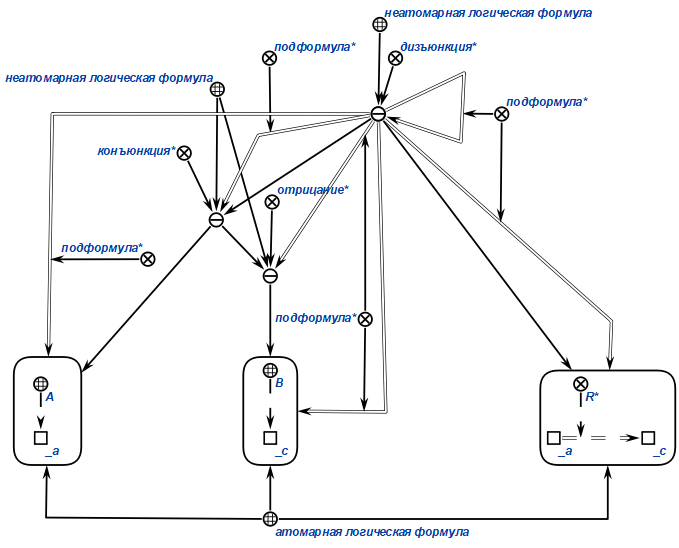
\includegraphics[scale=0.8]{author/part2/figures/logic/subformula.png}
	\caption{Формализация примера подформулы}
	\label{fig:modus_ponens}
\end{figure}

\textbf{\textit{утверждение}} -- это \textit{семантическая окрестность} некоторой \textit{логической формулы}, в которую входит полный текст этой \textit{логической формулы}, а также факт принадлежности этой \textit{логической формулы} некоторой \textit{формальной теории}.

Знак \textit{логической формулы}, семантическая окрестность которой представляет собой утверждение, является \textit{главным ключевым sc-элементом\scnrolesign} в рамках этого \textbf{\textit{утверждения}}. Знаки понятий соответствующей \textit{предметной области}, которые входят в состав какой-либо \textit{подформулы*} указанной \textit{логической формулы}, будут \textit{ключевыми sc-элементами\scnrolesign} в рамках этого \textbf{\textit{утверждения}}.
	
Полный текст некоторой \textit{логической формулы} включает в себя:
\begin{textitemize}
	\item{знак самой этой \textit{логической формулы}};
	\item{знаки всех ее \textit{подформул*}};
	\item{элементы всех \textit{логических формул}, знаки которых попали в данную структуру;}
	\item{все пары принадлежности, связывающие \textit{логические формулы}, знаки которых попали в данную структуру, с их компонентами.}
\end{textitemize}

Таким образом, факт принадлежности (истинности) логической формулы нескольким \textit{формальным теориям} будет порождать новое утверждение для каждой такой \textit{формальной теории}. Текст \textbf{\textit{утверждения}} входит в состав \textit{логической онтологии}, соответствующей \textit{предметной области}, на которой интерпретируется \textit{главный ключевой sc-элемент\scnrolesign} данного утверждения.

Правило идентификации экземпляров. \textbf{\textit{утверждения}} в рамках \textit{Русского языка} именуются по следующим правилам:
\begin{textitemize}
	\item{в начале идентификатора пишется сокращение \textbf{Утв.};}
	\item{далее в круглых скобках через точку с запятой перечисляются основные идентификаторы \textit{ключевых \mbox{sc-элементов}\scnrolesign} данного \textbf{\textit{утверждения}}. Порядок определяется в каждом конкретном случае в зависимости от того, свойства каких из этих \textit{понятий} описывает данное \textbf{\textit{утверждение}} в большей или меньшей степени.}
\end{textitemize}

%\scntext{описание примера}{\textit{Утв. (параллельность*; секущая*)}}
Могут быть исключения для \textbf{\textit{утверждений}}, названия которых закрепились исторически, например, \textit{Теорема Пифагора}, \textit{Аксиома о прямой и точке}.


%\scnrelfrom{описание примера}{\scnfilescg{figures/sd_logical_formulas/statement.png}}
%Утверждение показывает, что соответствующие углы при пересечении параллельных прямых секущей равны.

\textbf{\textit{Определение}} -- это \textit{утверждение}, \textit{главным ключевым sc-элементом\scnrolesign} которого является связка \textit{эквиваленции*}, однозначно определяющая некоторое понятие на основе других понятий.

Каждое определение имеет ровно один \textit{ключевой sc-элемент\scnrolesign} (не считая \textit{главного ключевого sc-элемента\scnrolesign}).

Для одного и того же понятия в рамках одной \textit{формальной теории} может существовать несколько \textit{утверждений об эквиваленции*}, однозначно задающих некоторое понятие на основе других, однако только одно такое \textit{утверждение} в рамках этой \textit{формальной теории} может быть отмечено как \textbf{\textit{определение}}. Остальные \textit{утверждения об эквиваленции*} могут трактоваться как \textit{пояснения} данного понятия.

Правило идентификации экземпляров. \textbf{\textit{определения}} в рамках \textit{Русского языка} именуются по следующим правилам:
\begin{textitemize}
	\item{в начале идентификатора пишется сокращение \textbf{Опр.};}
	\item{далее в круглых скобках через точку с запятой записывается основной идентификатор  \textit{ключевого sc-элемента\scnrolesign} данного \textbf{\textit{определения}}.}
\end{textitemize}


%\scntext{описание примера}{\textit{Опр. (ромб)}}
%\scnrelfrom{описание примера}{\scnfilescg{figures/sd_logical_formulas/definition.png}}
%\scnnote{Определение показывает, что ромб — это четырёхугольник, у которого все стороны равны.}
\begin{SCn}
\scnheader{общезначимая логическая формула}
\scnidtf{тождественно истинная логическая формула}
\scnsubset{выполнимая логическая формула}
\scnsubset{тавтология}
\end{SCn}
% Вагин, дедукция и обобщение в системах принятия решений
\textbf{\textit{Общезначимая логическая формула}} -- это \textit{логическая формула}, для которой не существует \textit{формальной теории}, в рамках которой она была бы ложной с учетом истинности и ложности всех ее \textit{подформул*} в рамках этой же \textit{формальной теории}.

\begin{figure}[http]
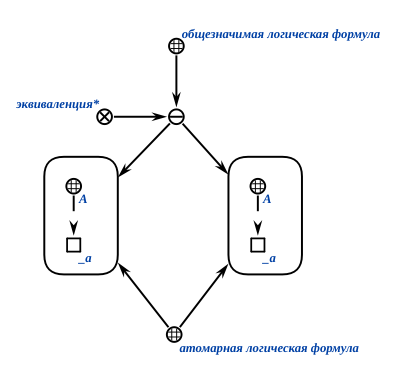
\includegraphics[scale=0.8]{author/part2/figures/logic/valid_formula.png}
\caption{Формализация закона тождества}
\label{fig:valid_formula}
\end{figure}

\begin{SCn}
\scnheader{противоречивая логическая формула}
\scnidtf{тождественно ложная логическая формула}
\scnsubset{невыполнимая логическая формула}
\scnsubset{тавтология}
\end{SCn}
% Вагин, дедукция и обобщение в системах принятия решений
\textbf{\textit{Противоречивая логическая формула}} -- это \textit{логическая формула}, для которой не существует \textit{формальной теории}, в рамках которой она была бы истинной с учетом истинности и ложности всех ее \textit{подформул*} в рамках этой же \textit{формальной теории}.

\begin{figure}[http]
	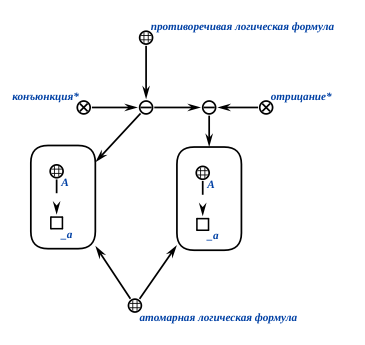
\includegraphics[scale=0.8]{author/part2/figures/logic/contradiction_formula.png}
	\caption{Формализация закона противоречия}
	\label{fig:contradiction_formula}
\end{figure}

\begin{SCn}
\scnheader{нейтральная логическая формула}
\scnsubset{выполнимая логическая формула}
\end{SCn}

\textbf{\textit{нейтральная логическая формула}} -- это \textit{логическая формула}, для которой существует хотя бы одна \textit{формальная теория}, в рамках которой эта формула ложна, и хотя бы одна \textit{формальная теория}, в рамках которой эта формула истинна.

\begin{figure}[http]
	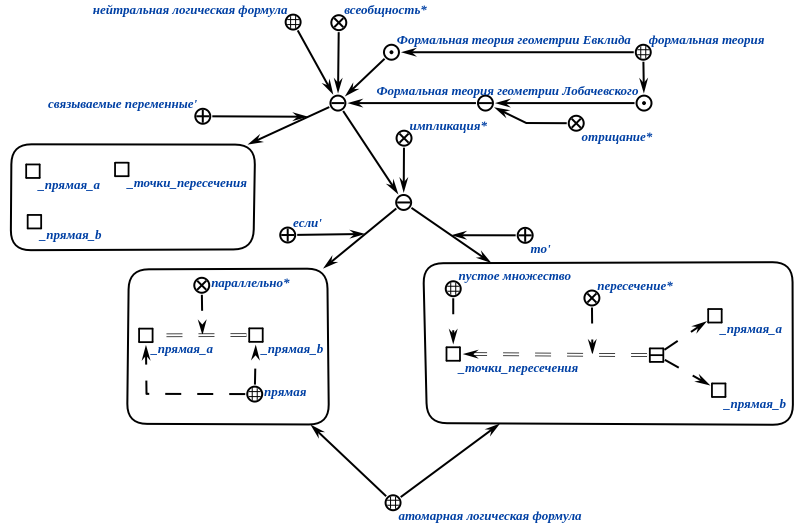
\includegraphics[scale=0.8]{author/part2/figures/logic/neutral_formula.png}
	\caption{Формализация нейтральной логической формулы}
	\label{fig:neutral_formula}
\end{figure}

В евклидовой геометрии в плоскости через точку, не лежащую на данной прямой, можно провести одну и только одну прямую, параллельную данной. В геометрии Лобачевского данный постулат является ложным.
В сферической геометрии все прямые пересекаются.

\begin{SCn}
\scnheader{непротиворечивая логическая формула}
\scnidtf{выполнимая логическая формула}
\begin{scnreltoset}{объединение}
	\scnitem{нейтральная логическая формула}
	\scnitem{общезначимая логическая формула}
\end{scnreltoset}
\end{SCn}

\textbf{\textit{непротиворечивая логическая формула}} -- это \textit{логическая формула}, для которой существует хотя бы одна \textit{формальная теория}, в рамках которой эта формула истинна.

\begin{SCn}
\scnheader{необщезначимая логическая формула}
\scnidtf{невыполнимая логическая формула}
\begin{scnreltoset}{объединение}
	\scnitem{нейтральная логическая формула}
	\scnitem{противоречивая логическая формула}
\end{scnreltoset}
\end{SCn}

\textbf{\textit{необщезначимая логическая формула}} -- это \textit{логическая формула}, для которой существует хотя бы одна \textit{формальная теория}, в рамках которой эта формула ложна.

Тавтология -- это \textit{логическая формула}, которая является либо только истинной, либо только ложной в рамках всех \textit{формальных теорий}, в которых можно установить ее истинность или ложность.
Тавтология -- это такая \textit{логическая формула}, которая является либо \textit{общезначимой логической формулой}, либо \textit{противоречивой логической формулой}.

\begin{SCn}
\scnheader{логическая связка*}
\scnidtf{неатомарная логическая формула}
\scnidtf{логический оператор*}
\scnidtf{пропозициональная связка*}
\scniselement{класс связок разной мощности}
\scnrelto{семейство подмножеств}{неатомарное высказывание}
\end{SCn}

\textbf{\textit{логическая связка*}} -- это отношение (класс связок), связками которого являются \textit{высказывания}, а областью определения которого является множество \textit{высказываний}, при этом само это отношение и некоторые его подмножества могут быть \textit{классами связок разной мощности}.

\begin{SCn}
\scnheader{конъюнкция*}
\scnidtf{логическое и*}
\scnidtf{логическое умножение*}
\scnsubset{логическая связка*}
\scniselement{неориентированное отношение}
\scniselement{класс связок разной мощности}
\scniselement{неунарное отношение}
\scnrelfrom{область определения}{логическая формула}
\end{SCn}

\textbf{\textit{конъюнкция*}} -- это множество конъюнктивных \textit{высказываний}, каждое из которых истинно в рамках некоторой \textit{формальной теории} только в том случае, когда все его компоненты истинны в рамках этой же \textit{формальной теории}. \textit{конъюнкция*} атомарных формул может быть заменена на атомарную формулу, полученную путём объединения исходных атомарных формул.

\begin{figure}[http]
	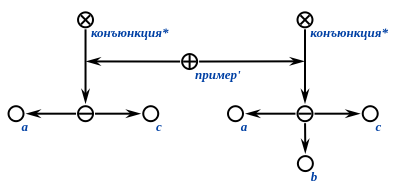
\includegraphics[scale=0.8]{author/part2/figures/logic/conjunction.png}
	\caption{Формализация примера конъюнкции}
	\label{fig:conjunction}
\end{figure}

\begin{figure}[http]
	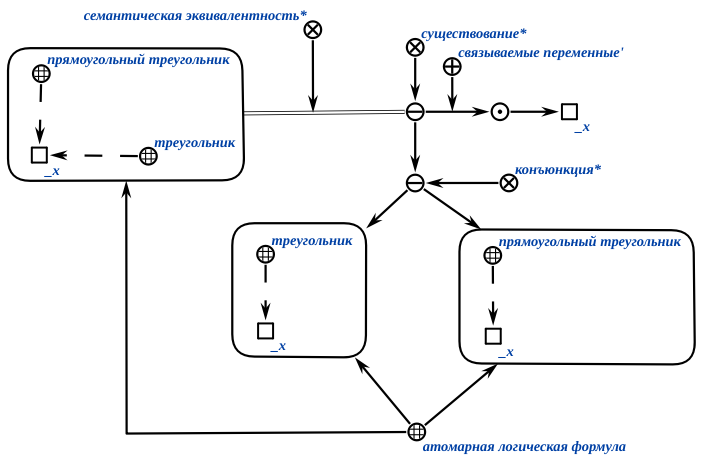
\includegraphics[scale=0.8]{author/part2/figures/logic/conjunction_triangles.png}
	\caption{Формализация примера конъюнкции в геометрии}
	\label{fig:conjunction_triangles}
	\scnexplanation{Данные конструкции эквивалентны по принципу $\exists x T(x) \land \exists x PT(x) \ \Longrightarrow \ \exists x (T(x) \land PT(x))$}
\end{figure}

\begin{SCn}
\scnheader{дизъюнкция*}
\scnidtf{логическое или*}
\scnidtf{логическое сложение*}
\scnidtf{включающее или*}
\scnsubset{логическая связка*}
\scniselement{неориентированное отношение}
\scniselement{класс связок разной мощности}
\scniselement{неунарное отношение}
\scnrelfrom{область определения}{логическая формула}
\end{SCn}

\textbf{\textit{дизъюнкция*}} -- это множество дизъюнктивных \textit{высказываний}, каждое из которых истинно в рамках некоторой \textit{формальной теории} только в том случае, когда хотя бы один его компонент является истинным в рамках этой же \textit{формальной теории}.

\begin{figure}[http]
	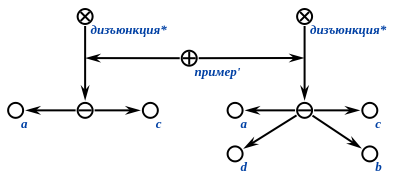
\includegraphics[scale=0.8]{author/part2/figures/logic/disjunction.png}
	\caption{Формализация примера дизъюнкции}
	\label{fig:disjunction}
\end{figure}

\begin{SCn}
\scnheader{отрицание*}
\scnsubset{логическая связка*}
\scnsubset{синглетон}
\scniselement{унарное отношение}
\scnrelfrom{область определения}{логическая формула}
\end{SCn}

\textbf{\textit{отрицание*}} -- это множество \textit{высказываний} об отрицании, каждое из которых истинно в рамках некоторой \textit{формальной теории} только в том случае, когда его единственный элемент является ложным в рамках этой же \textit{формальной теории}.

\begin{figure}[http]
	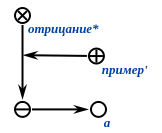
\includegraphics[scale=0.8]{author/part2/figures/logic/negation.png}
	\caption{Формализация примера отрицания}
	\label{fig:negation}
\end{figure}

\begin{SCn}
\scnheader{строгая дизъюнкция*}
\scnidtf{сложение по модулю 2*}
\scnidtf{исключающее или*}
\scnidtf{альтернатива*}
\scnsubset{логическая связка*}
\scniselement{неориентированное отношение}
\scniselement{класс связок разной мощности}
\end{SCn}

\textbf{\textit{строгая дизъюнкция*}} -- это множество строго дизъюнктивных \textit{высказываний}, каждое из которых истинно в рамках некоторой \textit{формальной теории} только в том случае, когда ровно один его компонент является истинным в рамках этой же \textit{формальной теории}.

\begin{figure}[http]
	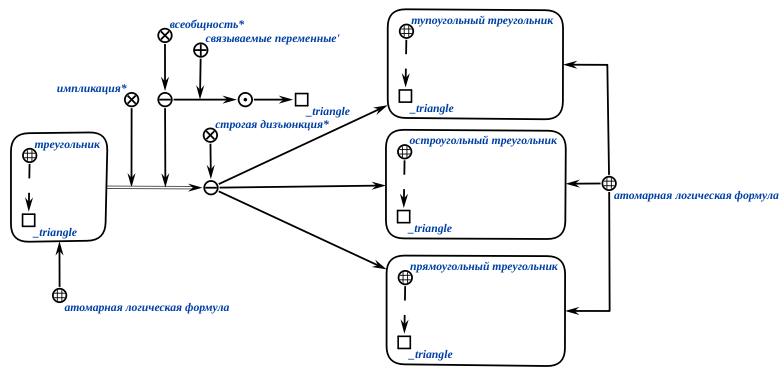
\includegraphics[scale=0.8]{author/part2/figures/logic/strict_disjunction_triangle.png}
	\caption{Формализация примера строгой дизъюнкции в геометрии}
	\label{fig:strict_disjunction_triangle}
\end{figure}
	\scnexplanation{Данная неатомарная логическая формула содержит следующую информацию: для любых переменных \_triangle если \_triangle является треугольником, то \_triangle является или тупоугольным треугольником, или остроугольным треугольником, или прямоугольным треугольником.}

\begin{figure}[http]
	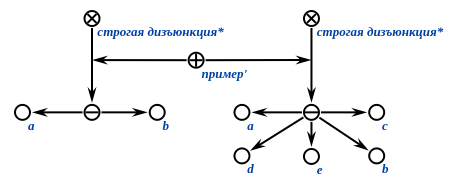
\includegraphics[scale=0.8]{author/part2/figures/logic/strictDisjunction.png}
	\caption{Формализация примера строгой дизъюнкции}
	\label{fig:strict_disjunction}
\end{figure}


\textbf{\textit{строгая дизъюнкция*}} может быть представлена как \textit{дизъюнкция} \textit{конъюнкции} \textit{отрицания} первой логической формулы и второй логической формулы и \textit{конъюнкции} первой логической формулы и \textit{отрицания} второй логической формулы. Также она может быть представлена и ввиде \textit{конъюнкции} \textit{дизъюнкций} двух логических формул и их \textit{отрицаний}.

\begin{figure}[http]
	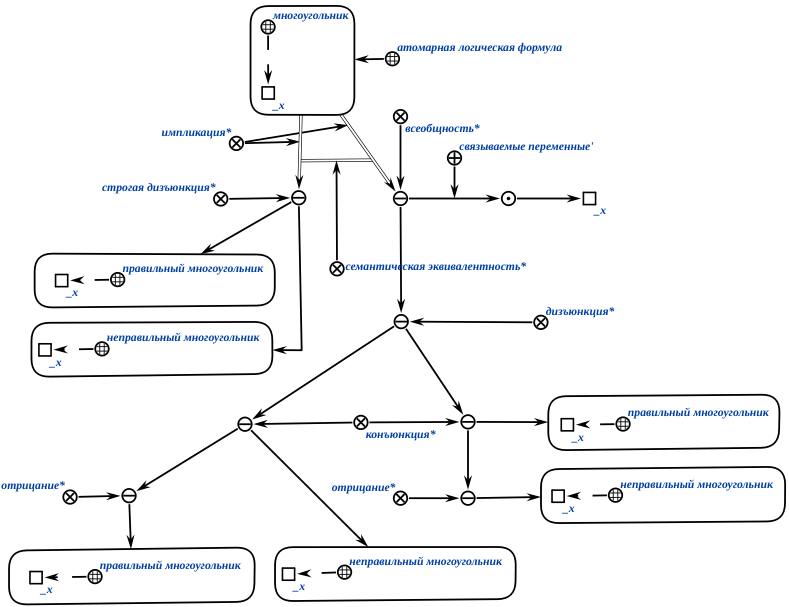
\includegraphics[scale=0.8]{author/part2/figures/logic/strict_disjunction_representation.png}
	\caption{Формализация примера строгой дизъюнкции}
	\label{fig:strict_disjunction_representation}
\end{figure}

\begin{SCn}
\scnheader{импликация*}
\scnidtf{логическое следование*}
\scnsubset{логическая связка*}
\scniselement{бинарное отношение}
\scniselement{ориентированное отношение}
\scnrelfrom{область определения}{логическая формула}
\end{SCn}

\textbf{\textit{импликация*}} -- это множество импликативных \textit{неатомарных высказываний}, каждое из которых состоит из посылки (первый компонент \textit{высказывания}) и следствия (второй компонент \textit{высказывания}).

Каждое импликативное \textit{высказывание} ложно в рамках некоторой \textit{формальной теории} в том случае, когда его посылка истинна, а заключение ложно в рамках этой же \textit{формальной теории}. В других случаях такое \textit{высказывание} истинно.

По умолчанию на все переменные, входящие в обе части высказывания об \textbf{\textit{импликации*}} (или хотя бы одну из \textit{подформул*} каждой части) неявно накладывается квантор \textit{всеобщности*}, при условии, что эти переменные не связаны другим \textit{квантором}, указанным явно.

\begin{figure}[http]
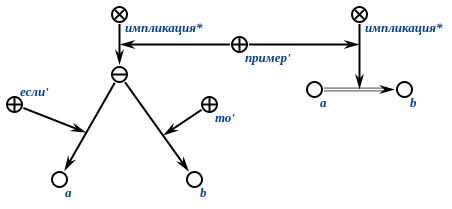
\includegraphics[scale=0.8]{author/part2/figures/logic/implication.png}
\caption{Формализация примера импликации}
\label{fig:implication}
\end{figure}

\textbf{\textit{импликация*}} может быть представлена как \textit{дизъюнкция} \textit{отрицания} первой логической формулы и второй логической формулы или же как \textit{отрицание} \textit{конъюнкции} первой логической формулы и \textit{отрицания} второй логической формулы.

\begin{figure}[http]
	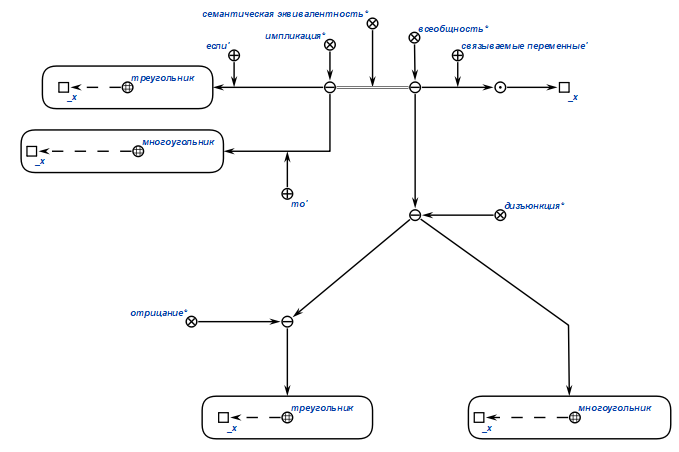
\includegraphics[scale=0.8]{author/part2/figures/logic/implication_representation.png}
	\caption{Формализация примера импликации}
	\label{fig:implication_representation}
\end{figure}

\begin{figure}[http]
	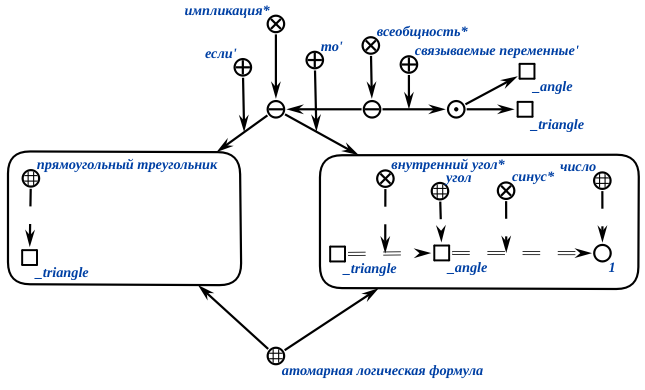
\includegraphics[scale=0.8]{author/part2/figures/logic/implication_triangle.png}
	\caption{Формализация примера импликации}
	\label{fig:implication_triangle}
	\scnexplanation{Данная неатомарная логическая формула содержит следующую информацию: для любых переменных \_triangle и \_angle если \_triangle является прямоугольным треугольником, то синус его внутреннего угла \_angle равен единице.}
\end{figure}

\begin{SCn}
\scnheader{если\scnrolesign}
\scnidtf{посылка\scnrolesign}
\scnsubset{1\scnrolesign}
\scniselement{ролевое отношение}
\end{SCn}

Если\scnrolesign -- это \textit{ролевое отношение}, используемое в связках \textit{импликации*} для указания посылки.

\begin{SCn}
\scnheader{то\scnrolesign}
\scnidtf{следствие\scnrolesign}
\scnsubset{2\scnrolesign}
\scniselement{ролевое отношение}
\end{SCn}

То\scnrolesign -- это \textit{ролевое отношение}, используемое в связках \textit{импликации*} для указания следствия.

\begin{SCn}
\scnheader{эквиваленция*}
\scnidtf{эквивалентность*}
\scnsubset{логическая связка*}
\scniselement{бинарное отношение}
\scniselement{неориентированное отношение}
\scnrelfrom{область определения}{логическая формула}
\end{SCn}

\textbf{\textit{эквиваленция*}} -- это множество \textit{высказываний} об эквивалентности, каждое из которых истинно в рамках некоторой \textit{формальной теории} только в тех случаях, когда оба его компонента одновременно либо истинны в рамках этой же \textit{формальной теории}, либо ложны.

По умолчанию на все переменные, входящие в обе части высказывания об \textbf{\textit{эквиваленции*}} (или хотя бы одну из \textit{подформул*} каждой части) неявно накладывается квантор \textit{всеобщности*}, при условии, что эти переменные не связаны другим \textit{квантором}, указанным явно.

\begin{figure}[http]
	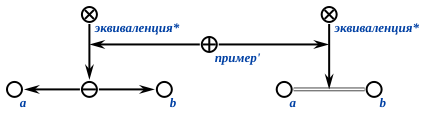
\includegraphics[scale=0.8]{author/part2/figures/logic/equivalent.png}
	\caption{Формализация примера эквиваленции}
	\label{fig:equivalent}
\end{figure}

\textbf{\textit{эквиваленция*}} двух логических формул может быть представлена как \textit{дизъюнкция} \textit{конъюнкции} этих двух логическх формул и \textit{конъюнкции} \textit{отрицаний} этих двух логических формул.

\begin{figure}[http]
	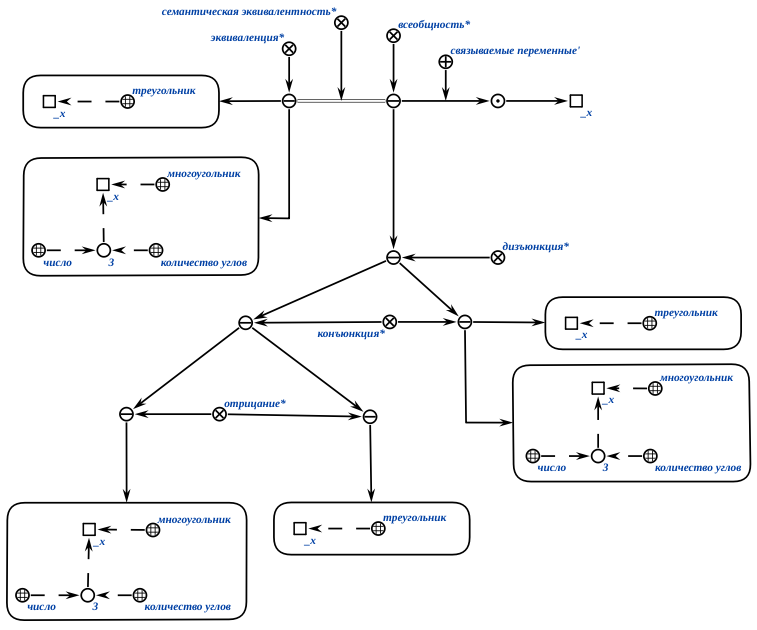
\includegraphics[scale=0.8]{author/part2/figures/logic/equivalence_representation.png}
	\caption{Формализация примера эквиваленции}
	\label{fig:equivalence_representation}
\end{figure}

\begin{SCn}
\scnheader{квантор}
\scnsubset{логическая связка*}
\end{SCn}

\textbf{\textit{квантор}} — это \textit{отношение}, каждая связка которой задает истинность множества \textit{логических формул}, входящих в ее состав, при выполнении дополнительных условий, связанных с некоторыми из переменных, входящих в состав этих \textit{логических формул}.

Будем говорить, что переменные связаны \textbf{\textit{квантором}} или попадают под область действия данного \textbf{\textit{квантора}} (имея в виду конкретную связку конкретного \textbf{\textit{квантора}}).

В состав каждой связки каждого \textbf{\textit{квантора}} входит \textit{атомарная формула}, являющаяся \textit{тривиальной структурой}, в которой перечислены переменные, связанные данным \textbf{\textit{квантором}}.

\begin{SCn}
\scnheader{всеобщность*}
\scnidtf{квантор всеобщности*}
\scnidtf{квантор общности*}
\scniselement{квантор}
\scniselement{ориентированное отношение}
\scniselement{класс связок разной мощности}
\end{SCn}

\textbf{\textit{всеобщность*}} -- это \textit{квантор}, для каждой связки которого, истинной в рамках некоторой \textit{формальной теории}, выполняется следующее утверждение: все формулы, входящие в состав этой связки истинны в рамках этой же \textit{формальной теории} при всех (любых) возможных значениях всех элементов множества \textit{связываемых переменных\scnrolesign} входящего в эту связку.

Каждая связка \textit{квантора} \textbf{\textit{всеобщность*}} может быть представлена как \textit{конъюнкция*} (потенциально бесконечная) исходных \textit{логических формул}, входящих в состав этой связки, в каждой из которых все \textit{связанные переменные\scnrolesign} заменены на их возможные значения.

Квантор \textbf{\textit{всеобщности*}} зачастую обозначается "$\forall$" \ и читается как "для всех"{}, "для каждого"{}, "для любого"{} или "все"{}, "каждый"{}, "любой".

\begin{figure}[http]
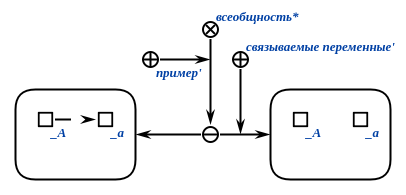
\includegraphics[scale=0.8]{author/part2/figures/logic/universality.png}
\caption{Формализация примера всеобщности}
\label{fig:universality}
\end{figure}

\begin{SCn}
\scnheader{формула существования}
\scnidtf{существование*}
\begin{scnreltoset}{разбиение}
	\scnitem{атомарная логическая формула}
	\scnitem{неатомарное существование*}
\end{scnreltoset}

\scnheader{неатомарное существование*}
\scnidtf{квантор неатомарного существования*}
\scniselement{квантор}
\scniselement{ориентированное отношение}
\scniselement{класс связок разной мощности}
\end{SCn}

\textbf{\textit{неатомарное существование*}} -- это \textit{квантор}, для каждой связки которого, истинной в рамках некоторой \textit{формальной теории}, выполняется следующее утверждение: существуют значения всех элементов множества \textit{связываемых переменных\scnrolesign} входящего в эту связку, такие, что все формулы, входящие в состав этой связки истинны в рамках этой же \textit{формальной теории}.

Каждая связка \textit{квантора} \textbf{\textit{неатомарное существование*}} может быть представлена как \textit{дизъюнкция*} (потенциально бесконечная) исходных \textit{логических формул}, входящих в состав этой связки, в каждой из которых все \textit{связанные переменные\scnrolesign} заменены на их возможные значения.

Квантор \textbf{\textit{существования*}} зачастую обозначается "$\exists$" \ и читается как "существует"{}, "для некоторого"{}, "найдется".

\begin{figure}[http]
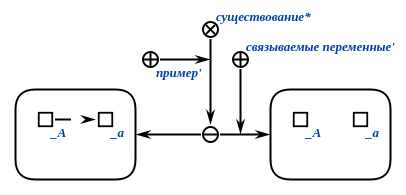
\includegraphics[scale=0.8]{author/part2/figures/logic/non_atomicExistence.png}
\caption{Формализация примера неатомарного существования}
\label{fig:non_atomic_existence}
\end{figure}

\begin{SCn}
\scnheader{число значений переменной}
\scniselement{параметр}
\end{SCn}

Каждый элемент \textit{параметра} \textbf{\textit{число значений переменной}} представляет собой класс ориентированных пар, первым компонентом которых является знак \textit{логической формулы}, вторым -- \textit{sc-переменная}, имеющая в рамках данной \textit{логической формулы} ограниченное известное число значений, при которых данная формула является истинной в рамках соответствующей \textit{формальной теории}.

Отметим, что в случае \textit{атомарной логической формулы} каждая такая связка связывает знак формулы и знак принадлежащей ей \textit{sc-переменной}, т.е. является, по сути, частным случаем пары принадлежности. В случае \textit{неатомарной логической формулы} указанная \textit{sc-переменная} может принадлежать любой из \textit{подформул*} исходной формулы.

\textit{измерением*} значения параметра \textbf{\textit{число значений переменной}} является некоторое \textit{число}, задающее количество значений \textit{sc-переменных} в рамках \textit{логической формулы}.

\begin{SCn}
\scnheader{кратность существования}
\scniselement{параметр}
\scnrelfrom{область определения параметра}{формула существования}
\scnhaselement{единственное существование}
\end{SCn}

Каждый элемент \textit{параметра} \textbf{\textit{кратность существования}} представляет собой класс логических \textit{формул существования}, для которых  при интерпретации на соответствующей \textit{предметной области} существует ограниченное общее для всех таких формул число комбинаций значений переменных, при которых указанные формулы являются истинными в рамках соответствующей \textit{формальной теории}.
\textit{измерением*} каждого значения \textbf{\textit{кратности существования}} является некоторое \textit{число}, задающее количество таких комбинаций.

\begin{SCn}
\scnheader{единственное существование}
\scnidtf{однократное существование}
\scnidtf{формула существования и единственности}
\end{SCn}

Единственное существование зачастую обозначается "$\exists!$" \ и читается как "существует и единственный".

\begin{SCn}
\scnheader{логическая формула и единственность}
\scnsubset{логическая формула}
\scnsubset{единственное существование}
\end{SCn}

Каждый элемент множества \textbf{\textit{логическая формула и единственность}} представляет собой \textit{логическую формулу} (\textit{атомарную} или \textit{неатомарную}), для которой дополнительно уточняется, что при ее интерпретации на некоторой предметной области существует только один набор значений переменных, входящих в эту формулу (или ее \textit{подформулы*}), при котором указанная логическая формула истинна в рамках \textit{формальной теории}, в которую входит данная \textit{предметная область}.


%\scnfilescg{figures/sd_logical_formulas/unique_existance.png}
%Данная формула показывает, что в рамках формальной теории геометрии Евклида существует только один прямоугольный треугольник с некоторым периметром, являющийся равнобедренным.

\textbf{\textit{связываемые переменные\scnrolesign}} -- это \textit{ролевое отношение}, которое связывает связку конкретного \textit{квантора} с множеством переменных, которые связаны этим квантором.

\textbf{\textit{открытая логическая формула}} -- это \textit{логическая формула}, в рамках которой (и всех ее \textit{подформул*}) существует хотя бы одна переменная, не связанная никаким \textit{квантором}.

\textbf{\textit{замкнутая логическая формула}} -- это \textit{логическая формула}, в рамках которой (и всех ее \textit{подформул*}) не существует переменных, не связанных каким-либо \textit{квантором}.

%\scnheader{Примеры неатомарных логических формул}
%\scneqtoset{\scgfileitem{figures/sd_logical_formulas/example_line_segment_sum.png}\\
%\scnrelfrom{описание примера}{
%\scnfilescg{figures/sd_logical_formulas/example_line_segment_sum_note.png}}
%\scnexplanation{AB+BC=AC}
%;
%\scgfileitem{figures/sd_logical_formulas/example_line_segment_diff.png}\\
%\scnrelfrom{описание примера}{
%\scnfilescg{figures/sd_logical_formulas/example_line_segment_diff_note.png}}
%\scnexplanation{AB-AC=CB}

\section{Смысловое представление логических формул и высказываний  в прикладных логиках}

\section{Смысловое представление логических формул и высказываний в неклассических логиках}

%\input{author/references}